\documentclass[]{article}

\usepackage{listings}
\usepackage{amsmath}
\usepackage{amssymb}
\usepackage{graphicx}
\usepackage{setspace}
\lstset{language=Python}

\title{Detecting Racism in Tweets : Progress Report}
\author{Fiete Botschen, Sean Noran}

\begin{document}

\maketitle

\onehalfspacing

\section{Goal Summary}
Our goal is to learn a supervised model that can detect racism in Tweets.

\section{Labeled Data Collection}

We are currently using a subset of a substantially large Twitter dataset. The data we used span over 20 days in January 2011 and 20 days in March 2015 and totals approximately 70 GB. This equates to nearly 30 million Tweets, including not only the Tweet itself but also various metadata pertaining to the Tweet, such as geolocation, Twitter account, number of times the Tweet was favorited, etc. The average Tweet contains about 30 characters and may contain links to images, news articles and other web content.

In addition to this available database of Tweets, we used a Twitter crawler to acquire a primarily racist dataset of Tweets by crawling a user that posts only racist content.

\subsection{Pre-Processing}
The first two datasets contain many Tweets in languages other than English. In order to isolate only English language Tweets, we filter our data by the language tag attached to each Tweet.

\subsection{Data Filtering}

The raw data is largely imbalanced; that is, racist Tweets occur infrequently. Thus generating an adequately large set of balanced data would be rather time-consuming. We therefore decide to filter the Tweets by words related to race. The list of words is not included in this report due to its explicit content.

For the dataset over January 2011, we filtered by explicit racial derogatory terms. In addition, we filtered the data by colors such as 'white' and 'black' and groups of people such as 'Mexicans' and 'Africans'. While many racist Tweets do include these terms, we found that most of the Tweets including these words were not considered racist, whereas the derogatory terms alone were better at isolating racism. This produced just over 70,000 Tweets.

For the dataset over March 2015, we filtered only by racial derogatory terms. This resulted in only around 10,000 Tweets to label.

\subsection{Data Labeling}

For the first dataset, we labeled 4000 Tweets manually ourselves and found 167 (4.175\%) of them to be racist.

For the second dataset, we labeled 4932 Tweets and found 426 (8.64\%) to be racist.

Because the labeling process was cumbersome for so few Tweets, we additionally decided to acquire data from a Twitter user who posts primarily racist content. Figure \ref{fig:word_count} shows the frequency of the most common words found in these Tweets, excluding the 100 most common English words. We labeled 54.17\% of these Tweets as racist, far exceeding the proportion of our previous labeled datasets.

\begin{figure}[h]
\label{fig:word_count}
\caption{Frequency of most common words in 6308 Tweets involving racist Twitter users (excluding 100 most common English words)}
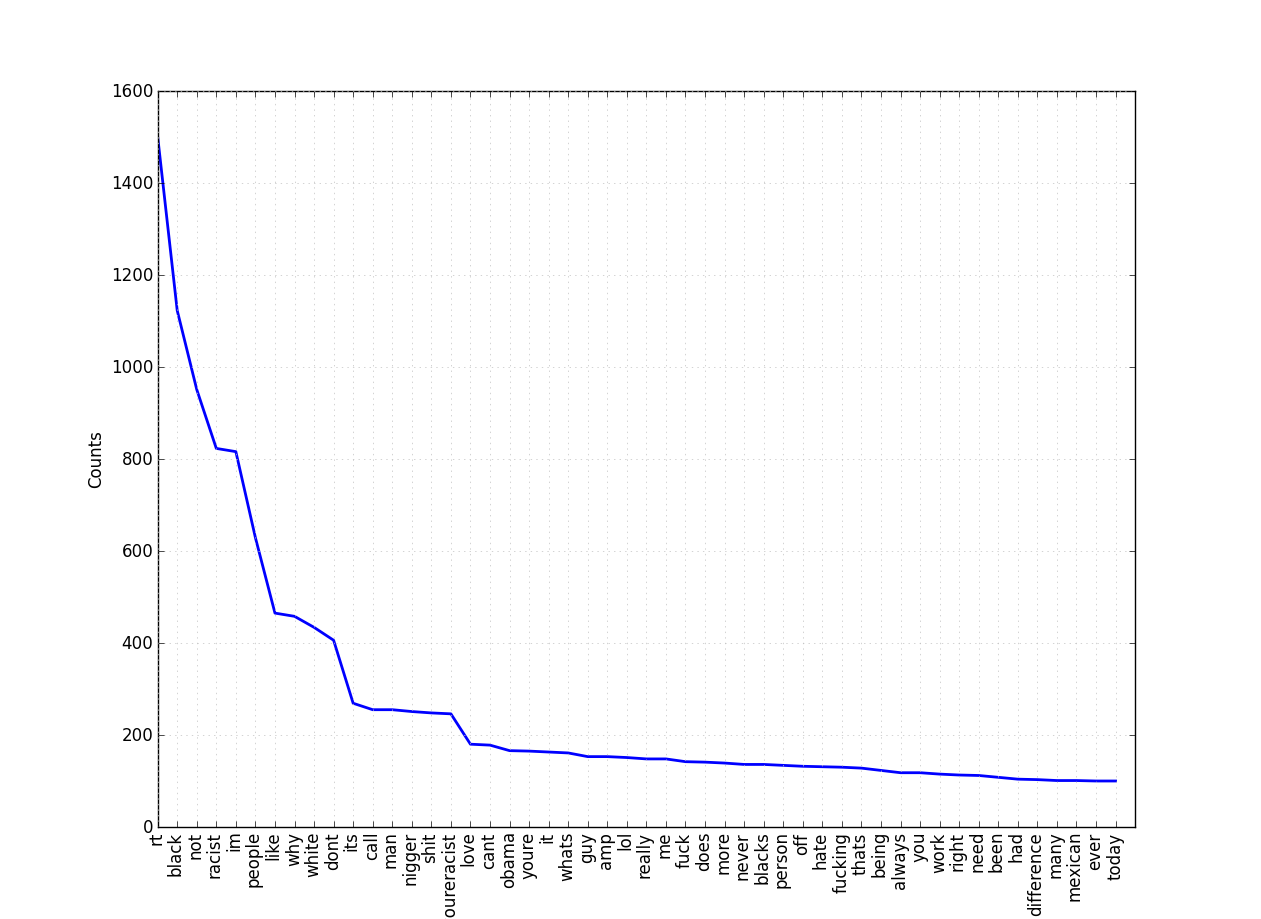
\includegraphics[width=8cm]{word_count}
\centering
\end{figure}

\subsection{Subjective Labeling}

One of the major questions involved in the data collection process is: What is racism? 

The U.S. Commission on Civil Rights defines racism as "any action or attitude, conscious or unconscious, that subordinates an individual or group based on skin colour or race. It can be enacted individually or institutionally"\footnote[1]{Racism In America and How to Combat It, U.S. Commission on Civil Rights, 1970}.

However, there is vast disagreement regarding how to define "race" and "subordinate". And indeed many alternative definitions of racism exist among various academic fields such as Sociology, Psychology, Political Science and Biology.

Because many people may disagree on which Tweets are racist, it would be better to define a confidence score as the percentage of people who said a given Tweet is racist. By this method, we would expect blatant racism to receive a confidence score close to 1, clearly non-racist Tweets to receive a score close to 0 and ambiguous Tweets to fall somewhere in between, close to 0.5.

However, it is also important to note that racism may be defined differently by different groups of people. In particular, an ethnic minority may find a certain Tweet to be racist, whereas a Caucasian may not see the racism in it.

Thus, if we are to collect data over a larger population of people, it would be important to account for many demographics. Additionally, we would want participants who themselves are not racist.

\section{Evaluation}
\subsection{Baseline Performance}

Our baseline algorithm labels as racist any Tweet which contains a word relevant to racism, specified in a pre-defined list of words. This algorithm does very poorly, because racist Tweets may not contain any such words. For instance:

	RT @DeadlySushi: @YesYoureRacist Instead of complaining about police fix youre neighborhoods first and stop doing crimes! Point the finger …
	
 (EXAMPLE) and, conversely, acceptable Tweets may contain several such words (EXAMPLE).


\subsection{Bag-of-Words Classification Results}

We evaluated three classifiers over binary bag-of-words features. Each model is trained on 4000 Tweets and evaluated on 2000 Tweets. In both cases, half of the Tweets are labeled as racist. For each Tweet, a binary feature is associated with each word in our vocabulary indicating whether the word appears in that Tweet. The top 100 most common English words are excluded. The results for each of three classifiers are shown below:

Naive Bayes: 72.889081832\%
Support Vector Machine: 72.9976123291\%
Random Forest: 73.258085522\%

We also found that if we vary the proportion of racist Tweets in our test dataset, the accuracy changes as follows:

200 non-racist, 2000 racist: ~55\%
2000 non-racist, 2000 racist: ~73\%
20000 non-racist, 2000 racist: ~88\%

This indicates that the models that we use tend to classify Tweets as non-racist more frequently than racist, despite the fact that our training data was balanced. This suggests that we need to improve feature engineering in order to achieve better accuracy.

\section{Timeline}

Our next steps involve

\begin{enumerate}
	\item Evaluating a bi-gram Naive Bayes model
	\item Reading additional existing research on similar work
	\item Feature Engineering
	\item Evaluating several classifiers
	\item Comparing our results to those of existing work
\end{enumerate} 

\end{document}